\documentclass[11pt,a4paper]{article}
\usepackage[margin=0.8in]{geometry}
\usepackage[utf8]{inputenc}
\usepackage{amsmath}
\usepackage{amsfonts}
\usepackage{amssymb}
\usepackage[hidelinks]{hyperref}
\usepackage{float}

%s comments
\usepackage{verbatim}

%inline graphs
\usepackage{wrapfig}
% multiple figures on line
\usepackage{subfig}

\usepackage{graphicx}
\graphicspath{ {img/} }

% Caption font size
% https://tex.stackexchange.com/questions/86120/font-size-of-figure-caption-header
\usepackage[font=scriptsize,labelfont=bf]{caption}

\setlength{\belowcaptionskip}{-10pt}
\setlength{\abovecaptionskip}{-5pt} % Chosen fairly arbitrarily


\usepackage{fancyhdr}
\pagestyle{fancy}
\lhead{\rightmark}
\chead{}
\rhead{SOFT354 - Parallel Computing and Distributed Systems}
\lfoot{\thepage}
\cfoot{}
\rfoot{Ben Lancaster 10424877}

\renewcommand{\subsectionmark}[1]{\markright{\thesubsection\ #1}}

\begin{document}

\begin{titlepage}
\begin{center}

\vspace*{3cm}
\Large
\textbf{SOFT354 - Parallel Computing and Distributed Systems}

\vspace{0.4cm}
\large
A comparison of the Discrete Fourier Transform algorithm implemented in CUDA and MPI.

\vspace{4cm}
\textbf{Ben Lancaster}\\
\today

\vspace{4cm}
\textbf{Abstract}\\
\small
My placement as a Firmware Engineer at Spirent, a world leader in GNSS simulators. Coming from a Computer Science I was up to speed on the programming aspect of firmware, however was lacking in experience of electronic lab equipment. Constant exposure to this new area of technology and equipment has greatly improved my knowledge in GNSS and embedded programming and has influenced my future career choices. I was chiefly responsible for writing a new programmable timer, implementing fan-control strategies and power calibration schemes, writing a driver to read in peripheral devices, provisioning a Linux hypervisor, and designing and implement a Linux USB driver.

\end{center}

\end{titlepage}

\renewcommand*\contentsname{Table of Contents}
\tableofcontents
\newpage

\section{Introduction}
This report discusses the implementation and performance of the Discrete Fourier Transform (DFT) algorithm in CUDA and MPI.

DFT is largely used in digital signal and image processing applications. 

In this report, I will be implementing the DFT to convert signals in the time domain to the frequency domain.

\begin{figure}[H]%
    \centering
    \subfloat[Time domain]{{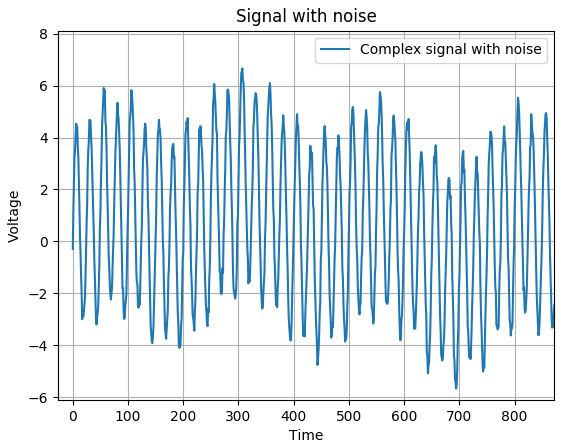
\includegraphics[width=7cm]{intro_signal} }}%
    \qquad
    \subfloat[Frequency domain]{{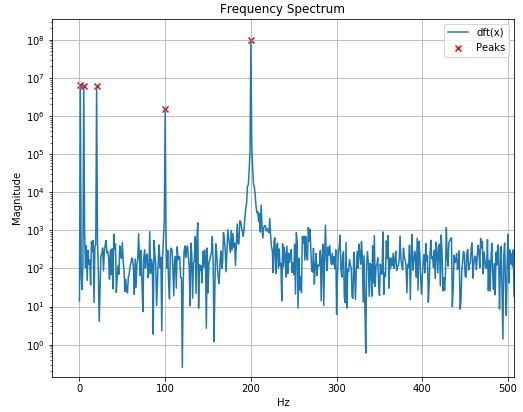
\includegraphics[width=7cm]{intro_dft} }}%
    \vspace{5pt}
    \caption{\textbf{Left:} A compound signal made up of 1, 5, 20, 100, and 200 Hz sine waves in the time domain. \textbf{Right:} Frequency domain representation showing high amplitude peaks for the 1, 5, 20, 100, and 200 Hz waveforms.}%
    \label{fig:gridwatch}%
\end{figure}

\section{Implementation}

\subsection{CUDA}
The CUDA implementation utilises a host device, typically a CPU, to retrieve the input samples from a file and store the resulting output. 

After reading the samples from a .csv file, the host allocates 2 global memory buffers on the device for the samples and output, and copies the input samples to the device. 

\begin{wrapfigure}{r}{0.4\textwidth}
\begin{center}
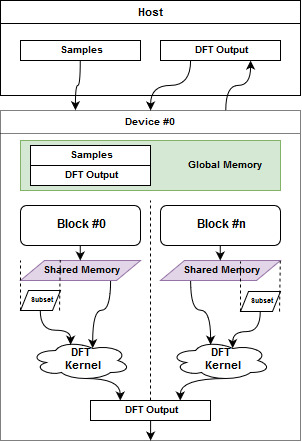
\includegraphics[scale=0.6]{cuda_impl1}
\end{center}
\caption{CUDA implementation control flow diagram showing memory }
\label{fig:cuda_impl1}
\end{wrapfigure}

As the input samples are 1D dimensional, kernels are launched with a 1D grids and blocks. 

The kernel assigns each output sample to a unique thread, identified by \textit{idx}. Each output sample must be calculated by iterating over the entire input sample vector. As the input sample size can contain many samples, the kernel will require many accesses to global memory. A technique, utilising the device's shared memory, is described in section \ref{sect:Dynamic Shared Memory} to reduce the number of global memory accesses.

Each thread writes it's result back into the global output buffer, which is then copied back from the device to the host.

\subsubsection{Dynamic Shared Memory} \label{sect:Dynamic Shared Memory}
As each operation on each sample requires values from all other samples, global memory accesses will be largest performance bottleneck. To reduce the amount of global memory accesses, I had the first thread of each block copy the complete global memory copy of the samples to a local shared memory buffer, which the DFT kernel would access instead of the global memory. 

On Compute Capability 2.0 devices, the maximum shared memory size per block is 48KB, meaning that if the kernel was launched with 1 block, it could access all 48KB of memory. If two blocks were used, each block would have 24KB of memory. 

To be able to fit the entire sample set in shared memory, I had to keep the maximum shared memory per block at it's highest by using as few blocks as possible. I used the maximum of 1024 threads per block to reduce the number of required blocks.  

\begin{wrapfigure}{r}{0.4\textwidth}
\begin{center}
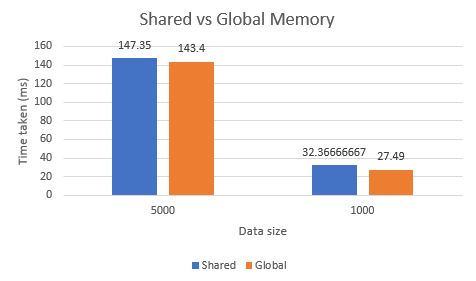
\includegraphics[scale=0.6]{shared_vs_global_graph}
\end{center}
\caption{Average kernel execution time using shared vs. global memory.}
\label{fig:shared_vs_global_graph}
\end{wrapfigure}

Using any number of 8-byte samples below 2048, which would use up to 2 blocks of 1024 threads and 24KB of shared memory, allows all samples for each block to fit into their shared memory. 

If using more than 2048 8-byte samples, resulting in using 3 or more blocks, results in the shared memory per block overflowing. The kernel handles this by pausing blocks that do not have enough shared memory ready, and running blocks that do have all their shared memory ready.

Even though we are accessing faster memory, it's size limitations causes resource availability delays when using larger data sets, which results in higher latency and lower performance. 

Figure \ref{fig:shared_vs_global_graph} shows the kernel execution time when using shared memory against global memory. We can see the global execution time is lower than shared memory. This is likely because the time taken for each block to copy the data set from global to shared (while other threads wait idle for the shared memory) is greater than the time of just accessing global memory.

\subsection{MPI}
The MPI implementation is similar to the CUDA kernel. Instead of each output sample being assigned to a thread, the output samples are split across a range of nodes. 

\begin{figure}[H]
\begin{center}
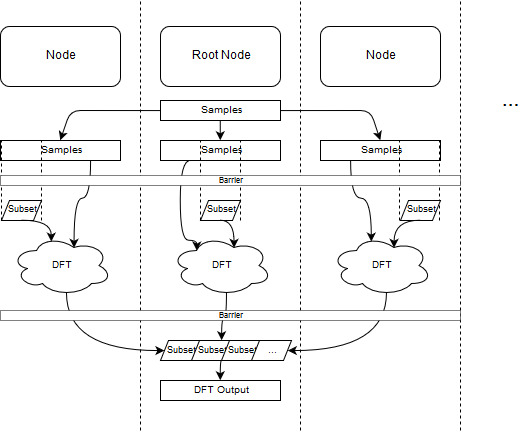
\includegraphics[scale=0.7]{mpi_impl1}
\end{center}
\caption{Control flow diagram for the MPI DFT algorithm.}
\label{fig:train10x}
\end{figure}

\section{Evaluation}
\subsection{Measuring Performance}
Performance metrics have been captured using Windows' `\textit{QueryPerformanceCounter}` and the `NSight Performance Analysis` tools. Helper macros, `\textit{TIME\_START}` and `\textit{TIME\_STOP}` are used to record timed code sections.

Key performance metrics that have been analysed are: Memory allocation time, MPI broadcast and Gather time, MPI DFT calculation time, CUDA kernel execution time, CUDA memory operations time, CUDA kernel occupancy, and number of blocked CUDA warps.

\subsection{MPI Node Count}
Note: All MPI performance measurements were taken on an Intel i5-6200U CPU clocked at 2.30 GHz.

When running MPI on a single machine, MPI will spawn multiple nodes (processes) that are subject the OS's scheduling strategy. In addition, depending on available CPU resources, like core count, MPI and the OS will assign CPU resources to each processes.

\begin{wrapfigure}{r}{0.5\textwidth}
\begin{center}
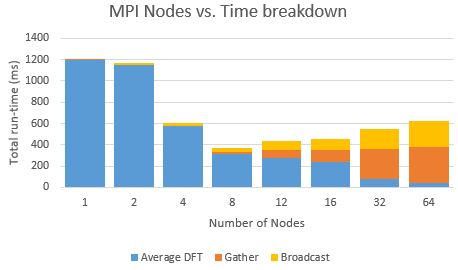
\includegraphics[scale=0.7]{mpi_eval_nodes}
\end{center}
\caption{Time breakdown of MPI program when run with different number of nodes.}
\label{fig:mpi_eval_nodes}
\end{wrapfigure}

Running on a 2 core, 4 thread CPU, with more MPI nodes than CPU threads, the OS will need to schedule each node with other running programs, which will reduce our MPI program's performance.

As seen in Figure \ref{fig:mpi_eval_nodes}, using few MPI nodes requires each node to work on more samples, which increases the average DFT calculate time. The small amount of nodes also means that little inter-process communication needs to take place to broadcast and gather the results.

Increasing the number of MPI nodes reduces the average DFT calculation time per node, as each node has fewer samples to work on, but inter-process communication is greatly increased. The MPI implementation uses blocking barrier communication messages to share and collect the results. With many nodes, it takes longer for MPI to synchronise the nodes resulting in longer total run-times.

From this, I predict that the optimum number of MPI nodes per machine for this algorithm is approximately 2x the total number of CPU threads.

\subsection{CUDA Threads Per Block}
Increasing the number of threads per block, whilst keeping the grid 1 dimensional, reduces the number of threads that need to write to shared memory. As discussed in \ref{sect:Dynamic Shared Memory}, the first node of each block copies the sample buffer from global memory to shared memory. This allows warps that would be waiting for shared memory to be ready, to become active and increase the occupancy of the kernel.

\begin{figure}[H]%
    \centering
    \subfloat[Time breakdown of CUDA program when run with different number of nodes.]{{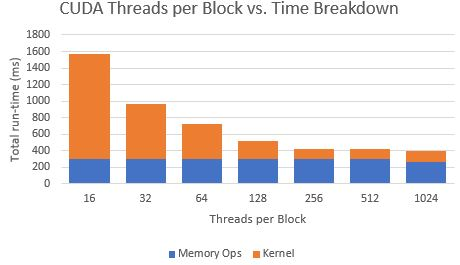
\includegraphics[width=7.5cm]{cuda_eval_threads} }}%
    \qquad
    \subfloat[Blocked Warps per block and Occupancy vs. Threads per Block.]{{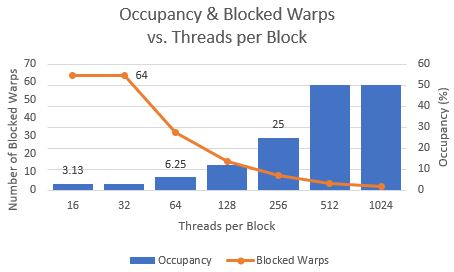
\includegraphics[width=7.5cm]{cuda_eval_occu} }}%
    \vspace{5pt}
    \caption{}%
    \label{fig:cuda_threads_per_block}%
\end{figure}

Figure \ref{fig:cuda_threads_per_block} (a) shows the kernel execution time decreasing as the number of threads per block increases. Figure \ref{fig:cuda_threads_per_block} (b) shows the number of blocked warps decreasing and occupancy increasing as the number of threads per block increases.

\section{Further Improvements}
\subsection{Sub-sample partitioning}
The current algorithmic approach to both MPI and CUDA solutions is to assign output samples to threads and nodes. The downside of this method is that each output sample must act upon all other input samples and is thus exponential in terms of computational complexity.

A solution to this is to assign a 'master' thread/node to each sample, then assign a unique thread for each input sample. The input sample threads would calculate their real and imaginary parts, which when required by a master thread, would reduce using a custom sum reduction method and then multiply by the input sample.

This solution would require twice as many threads/nodes as samples but would reduce the computation time by having each thread work out a partial solution. The master thread will not be required to calculate real and imaginary parts for all samples; it will just multiply the result from other threads by it's input sample value. The solution will still be of $O(n^2)$ complexity however it's execution time, for each sample, will be reduced linearly.

\subsection{CUDA - Increase Thread-block dimensions}
The current CUDA implementation uses a 1 dimension grid and block layout. Currently, my algorithm is limited to 1024*1024 threads (if assigning 1 thread per sample). As seen in section \ref{sect:Dynamic Shared Memory}, fewer blocks results in higher occupancy, so using 2 or 3 dimension thread blocks will increase our thread and sample limit without increasing the block count. 

\subsection{CUDA cuDoubleComplex}
My implementation uses 2 double variables, \textit{sum\_real} and \textit{sum\_imag}, to represent the real and imaginary parts of complex numbers.

Using CUDA's built in \textit{cudoubleComplex} type will likely increase performance on a per-instruction basis. CUDA provides built in intrinsic functions for double and complex numbers, like \textit{cuCmul}, that map directly to device instructions.

\newpage
\section{Conclusion}



\end{document}
